\chapter{Atividades desenvolvidas}
\label{cap:desenvolvimento}

Nos primeiros dias como estagiário no LEMAF, foi necessário realizar treinamentos online para que entendesse como funcionava as principais tecnologias utilizadas lá.
Forneceram uma licença na plataforma Alura para que aprendesse a utilizar o \textit{framework} VueJS e Spring e diversos livros sobre os processos \textit{Scrum} e banco de dados.

Um tutor foi designado para criar um quadro de tarefas que deveriam ser cumpridas para que tivesse o conhecimento básico para desenvolver os projetos.
Após terminar as tarefas, foi passado um projeto para que fosse possível praticar e verificar os conhecimentos obtidos.

Na sua grande maioria, os projetos do LEMAF são sistemas web\footnote{Sistemas web são soluções de software que podem ser acessados através de um navegador  em uma rede de computadores interna de uma empresa ou pela Internet.
}, constituídos de uma aplicação \textit{backend} e uma \textit{frontend}.

Durante o desenvolvimento, o \textit{backend} é, geralmente, compilado no computador do próprio desenvolvedor, porém quando há necessidade de serem feitos testes, é criado um servidor dentro da rede local para que possam ser efetuados os mesmos, sendo mais precisos por conta de estarem em um servidor.

A infraestrutura de servidores\footnote{Computadores físicos ou virtuais que executam e servem a aplicação} do LEMAF são servidores com diversas máquinas, todas rodando NGNIX\footnote{Disponivel em: https://www.nginx.com/} para prover as aplicações.

O \textit{frontend} seguia o mesmo processo do \textit{backend}, porém quando era enviado para alguma máquina externa, era criada alguma configuração para que o \textit{backend} servisse o \textit{frontend}, evitando assim problemas de CORS\footnote{CORS  (Cross-Origin Resource Sharing), é uma regra criada para segurança dos usuários ao  usar navegadores (\url{https://developer.mozilla.org/pt-BR/docs/Web/HTTP/Controle_Acesso_CORS})}.

Já o banco de dados\footnote{Estrutura de armazenamento de dados} era controlado por um DBA\footnote{Database Administrator, gerencia a estrutura do banco de dados, desde a escolha do gerenciador de banco de dados até a estrutura interna do mesmo.}, que criava e gerenciava toda a estrutura de banco, sendo somente necessário aos desenvolvedores discutir melhores soluções e criar demandas para os mesmos realizarem e contemplarem suas necessidades.

Para a maioria dos bancos era utilizada o SGBD\footnote{ Sistemas de Gestão de Base de Dados} Postgres\footnote{Disponivel em: https://www.postgresql.org/}, por conta de sua extensão POSTGIS que dava suporte a diversos tipos de dados relacionados a geometrias.

Como o foco do LEMAF é meio ambiente, o uso de mapas era recorrente na empresa, sendo necessário então obter um conhecimento básico sobre termos ambientais como APP e AUR.

\begin{quote}
    Área de preservação permanente - "área protegida, coberta ou não por vegetação nativa, com a função ambiental de preservar os recursos hídricos, a paisagem, a estabilidade geológica e a biodiversidade, facilitar o fluxo gênico de fauna e flora, proteger o solo e assegurar o bem-estar das populações humanas"\cite{brasil2012}
\end{quote}

\begin{quote}
    Áreas de Uso Restrito -  área localizada no interior de uma propriedade ou posse rural, delimitada nos termos do art. 12, com a função de assegurar o uso econômico de modo sustentável dos recursos naturais do imóvel rural, auxiliar a conservação e a reabilitação dos processos ecológicos e promover a conservação da biodiversidade, bem como o abrigo e a proteção de fauna silvestre e da flora nativa;
\cite{brasil2012}

\end{quote}

Durante o período de estagiário participou de todos squads, trabalhando com diversos times\footnote{Grupo de funcionários, geralmente formado por desenvolvedores, analistas de qualidade e Product Owners}, projetos e tecnologias.
E com isso, foi possível obter experiências com diversas tecnologias diferentes.
\begin{figure}[H]
\centering
\caption{Fluxo de aprendizado} %legenda
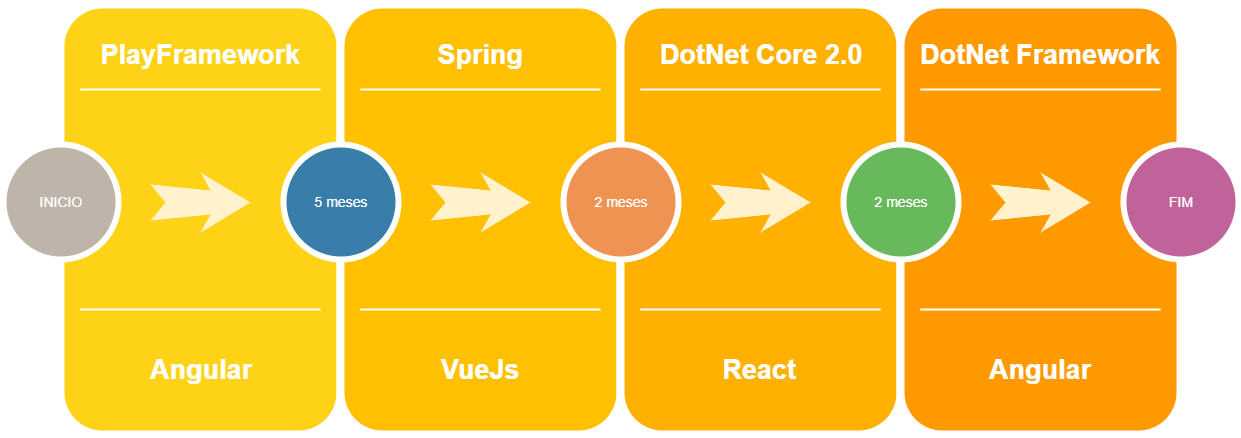
\includegraphics[scale=0.35]{fluxoAprendizado}\\  % o 0.9 indica 90% do tamanho original
% pdfLaTeX aceita figuras no formato PNG, JPG ou PDF
% figuras vetoriais podem ser exportadas para eps e depois convertidas para pdf usando epstopdf
\label{fig:exemplo} %rotulo para refencia
\end{figure}

\section{SICAR}

Em sua primeira equipe (Squad 1 - Carreta Furacão), tive como tecnologias necessárias JAVA (\textit{backend}) e Angular (Frontend) para evoluir os projetos do Cadastro Ambiental Rural, incluindo os projetos SICAR, Central do Responsável Técnico, Central do Proprietário, PRA-OFF.

Meu trabalho nesta equipe era desenvolver novas funcionalidades no sistema, como inserir novos dados no arquivo .PRA gerado pelo PRA-OFF, criptografa-lo e descriptografa-lo nas centrais.

Foi onde também tive meu primeiro contato com o Banco de Dados, uma vez que ainda não havia feito a disciplina deste assunto e então não possuia domínio ou conhecimento necessário, porém sua equipe possuia desenvolvedores extremamente experientes e muito dispostos a ensinar.
tive diversas atividades onde era necessário a criação de comandos SQL e como todos passavam por validação do DBA, tinha recorrentemente que corrigir os mesmos, entendendo e aprendendo com meus erros.

Também tive o obstaculo de nunca ter utilizado alguma IDE, vinha programando em editores de texto desde o começo da graduação, então ao ter a necessidade de programar com eficiência, adotei o uso da IDE Eclipse, que já era utilizada pela equipe para desenvolvimento \textit{backend}.

O \textit{backend} era uma parte que conseguia entender, uma vez que já tinha experiências com JAVA graças a disciplina de Programação Orientada a Objetos e desenvolvimento Mobile, onde tive que desenvolver nativo para Android utilizando JAVA.

Para desenvolver e reproduzir o fluxo do sistema, foi necessário aprendizado sobre tecnologias relacionadas a georeferenciamento e mapas, como ARCGIS\footnote{Disponivel em: \url{https://www.arcgis.com/index.html}}, leaflet\footnote{Disponivel em: \url{https://leafletjs.com/}} e GEOSERVER\footnote{Disponivel em: \url{http://geoserver.org/}}.

ARCGIS era uma ferramenta para desenho e exibição de geometrias, sendo possível reproduzir desde fazendas pequenas(menos de 4 módulos fiscais\footnote{II - Pequena Propriedade - o imóvel rural:

a) de área compreendida entre 1 (um) e 4 (quatro) módulos fiscais;\cite{brasil1993}}) a áreas enormes.

A leaflet era a principal biblioteca utilizada para mapas dentro do LEMAF, uma vez que era grátis e eficiente, com ampla documentação e compatibilidade. A ferramenta era de extrema importância para os projetos.

E para que ficasse centralizado diversos recursos de mapa, como as geometrias de APP do estado do PArá, hidrografia e outros, era utilizado o GEOSERVER, uma ferramenta que armazenava, gerenciava e provia geometrias.

\begin{figure}[H]
\centering
\caption{SICAR-PA} %legenda
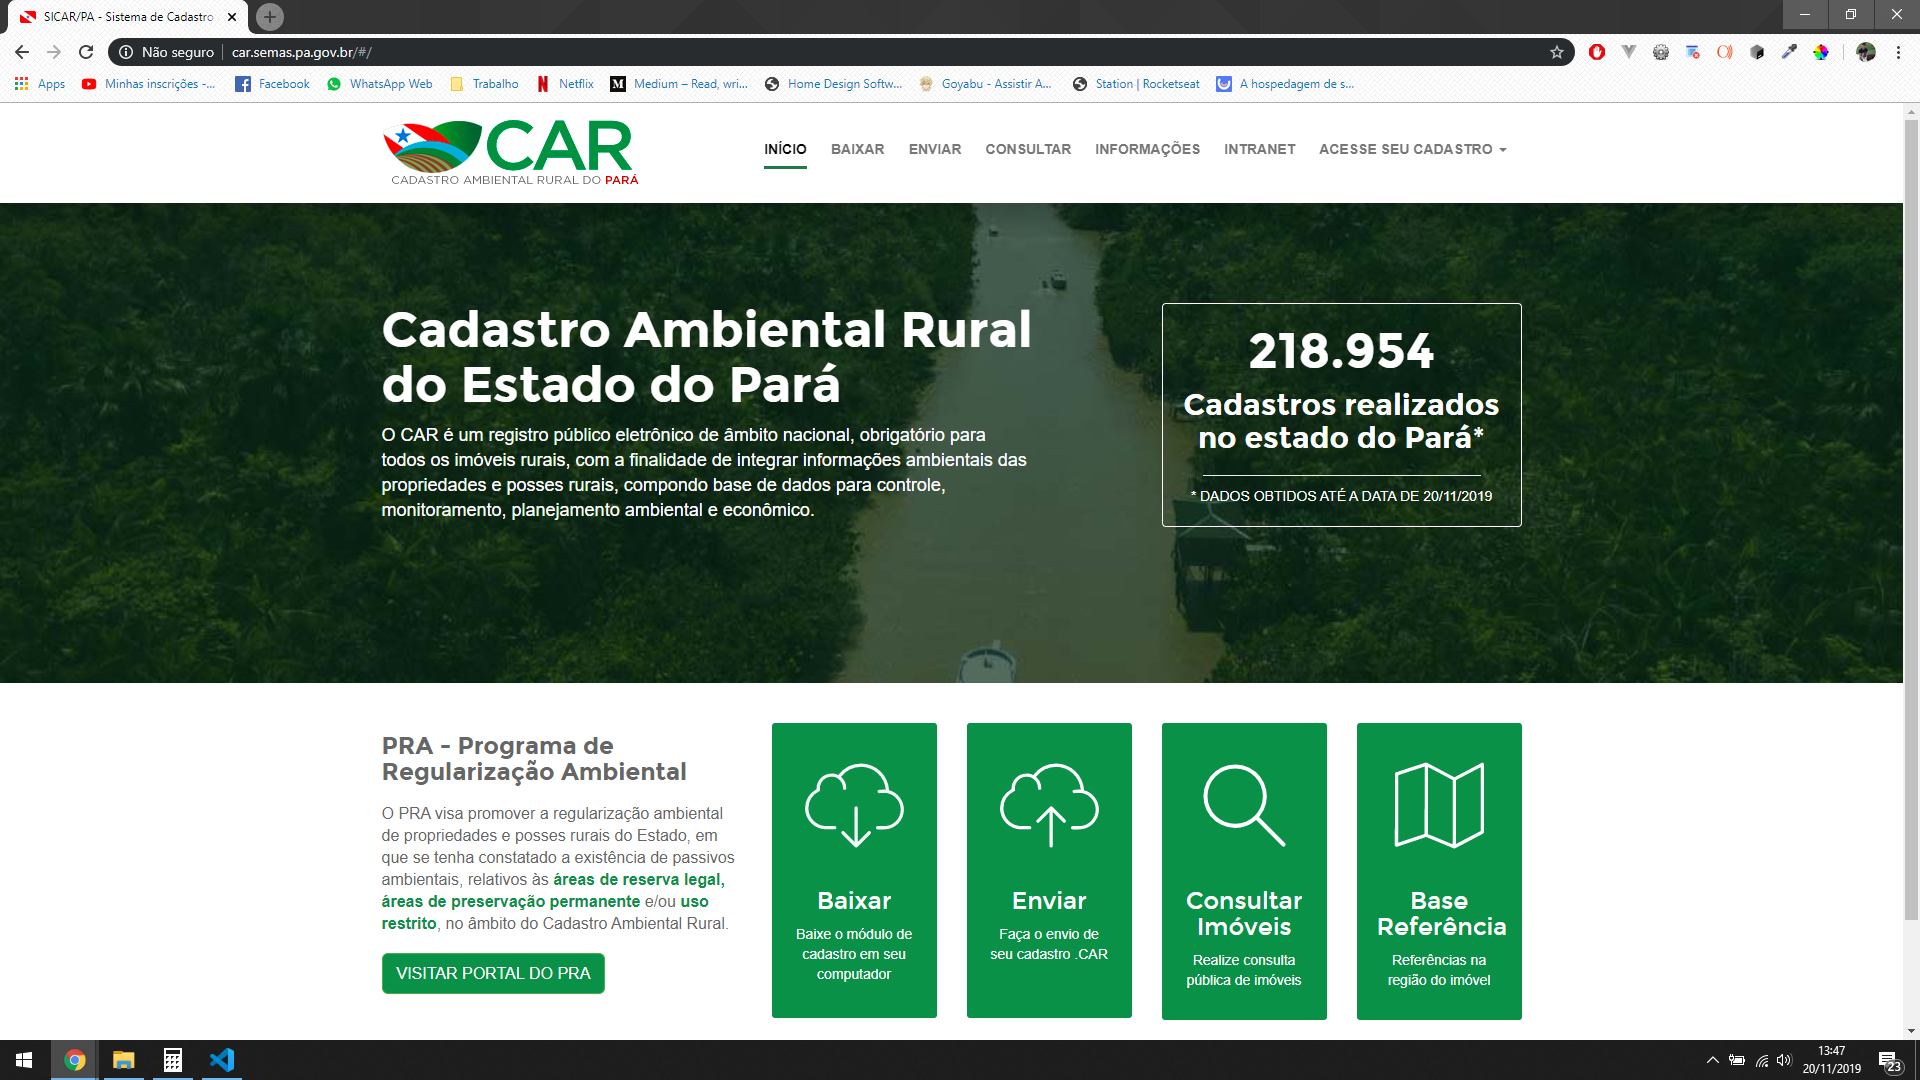
\includegraphics[scale=0.3]{SICAR}\\  % o 0.9 indica 90% do tamanho original
% pdfLaTeX aceita figuras no formato PNG, JPG ou PDF
% figuras vetoriais podem ser exportadas para eps e depois convertidas para pdf usando epstopdf
{\small Fonte: \url{http://car.semas.pa.gov.br/}} %Fonte da imagem
\label{fig:sicar} %rotulo para refencia
\end{figure}

O projeto do SICAR(Figura \ref{fig:sicar})\footnote{Sistema de Cadastro Ambiental Rural, uma plataforma relacionada ao governo e que gerenciava os cadastros.} tinha como objetivo informar e controlar os cadastros ambientais rurais feitos no estado do Pará, sendo necessárias algumas integrações com os módulos do SICAR federal e as Centrais ligadas ao PRA.

\begin{quote}
    Para adequação dos imóveis rurais à nova legislação, foi criado o Cadastramento
Ambiental Rural (CAR) como registro público eletrônico de âmbito nacional,
obrigatório para todos os imóveis rurais, com a finalidade de integrar as informações ambientais das propriedades e posses rurais, compondo base de dados
para controle, monitoramento, planejamento ambiental e econômico e combate
ao desmatamento. - \cite{de2015cadastro}
\end{quote}

\section{PRA}
\begin{figure}[H]
\centering
\caption{PRA-OFF} %legenda
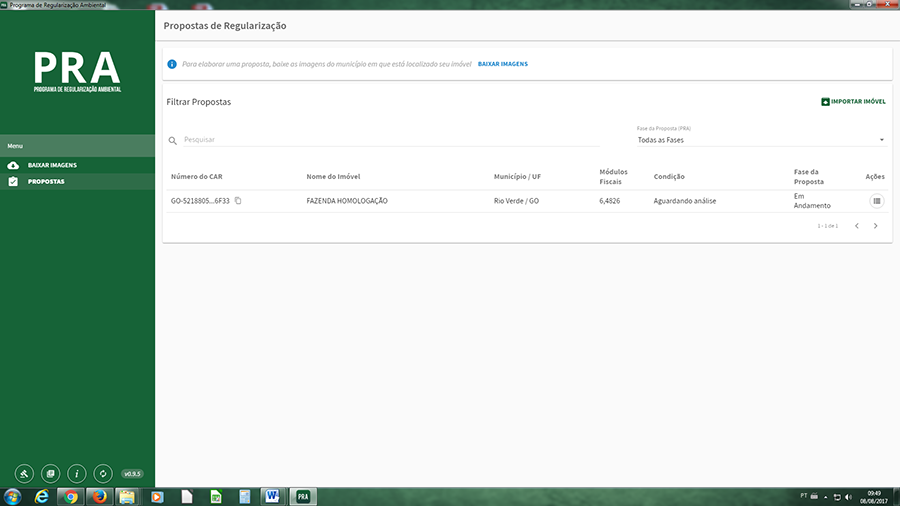
\includegraphics[scale=0.5]{pra-off}\\  % o 0.9 indica 90% do tamanho original
% pdfLaTeX aceita figuras no formato PNG, JPG ou PDF
% figuras vetoriais podem ser exportadas para eps e depois convertidas para pdf usando epstopdf
{\small Fonte: \url{http://www.cprh.pe.gov.br/Controle_Ambiental/Sistema%20Nacional%20de%20Cadastro%20Ambiental%20Rural%20-%20SICAR/PRA/43052%3B53356%3B480802%3B0%3B0.asp}} %Fonte da imagem
\label{fig:pra} %rotulo para refencia
\end{figure}

Já o projeto do PRA(Figura \ref{fig:pra})\footnote{Programa de regularização ambiental, responsável por regularizar situações de desmatamentos e outras inflações ambientais}, não eram possíveis tais integrações, pois ele era um módulo offline, sendo possível a utilização sem internet. Para o desenvolvimento do mesmo, foi necessário estudar sobre electron\footnote{Disponivel em: https://electronjs.org/}, uma ferramenta que possibilita criar módulos web em aplicações offline.

\section{Consulta Pública}
Após 5 meses a equipe foi dividida em duas e então foi feita uma redistribuição de projetos, quando fui alocado a tribo\footnote{Grupo de funcionários divido por equipes, gerenciado por um GP} Runners. Os projetos principais que contribui durante esse período foram o Consulta Pública - PARÁ e relatórios do PRA.

\begin{quote}
    O objetivo principal é promover as boas
    práticas de manejo florestal, por meio do enriquecimento das florestas secundárias
    remanescentes, localizadas fora das APPs, geralmente compondo a RL. - \cite{de2015cadastro}
\end{quote}
\begin{figure}[H]
\centering
\caption{Consulta publica} %legenda
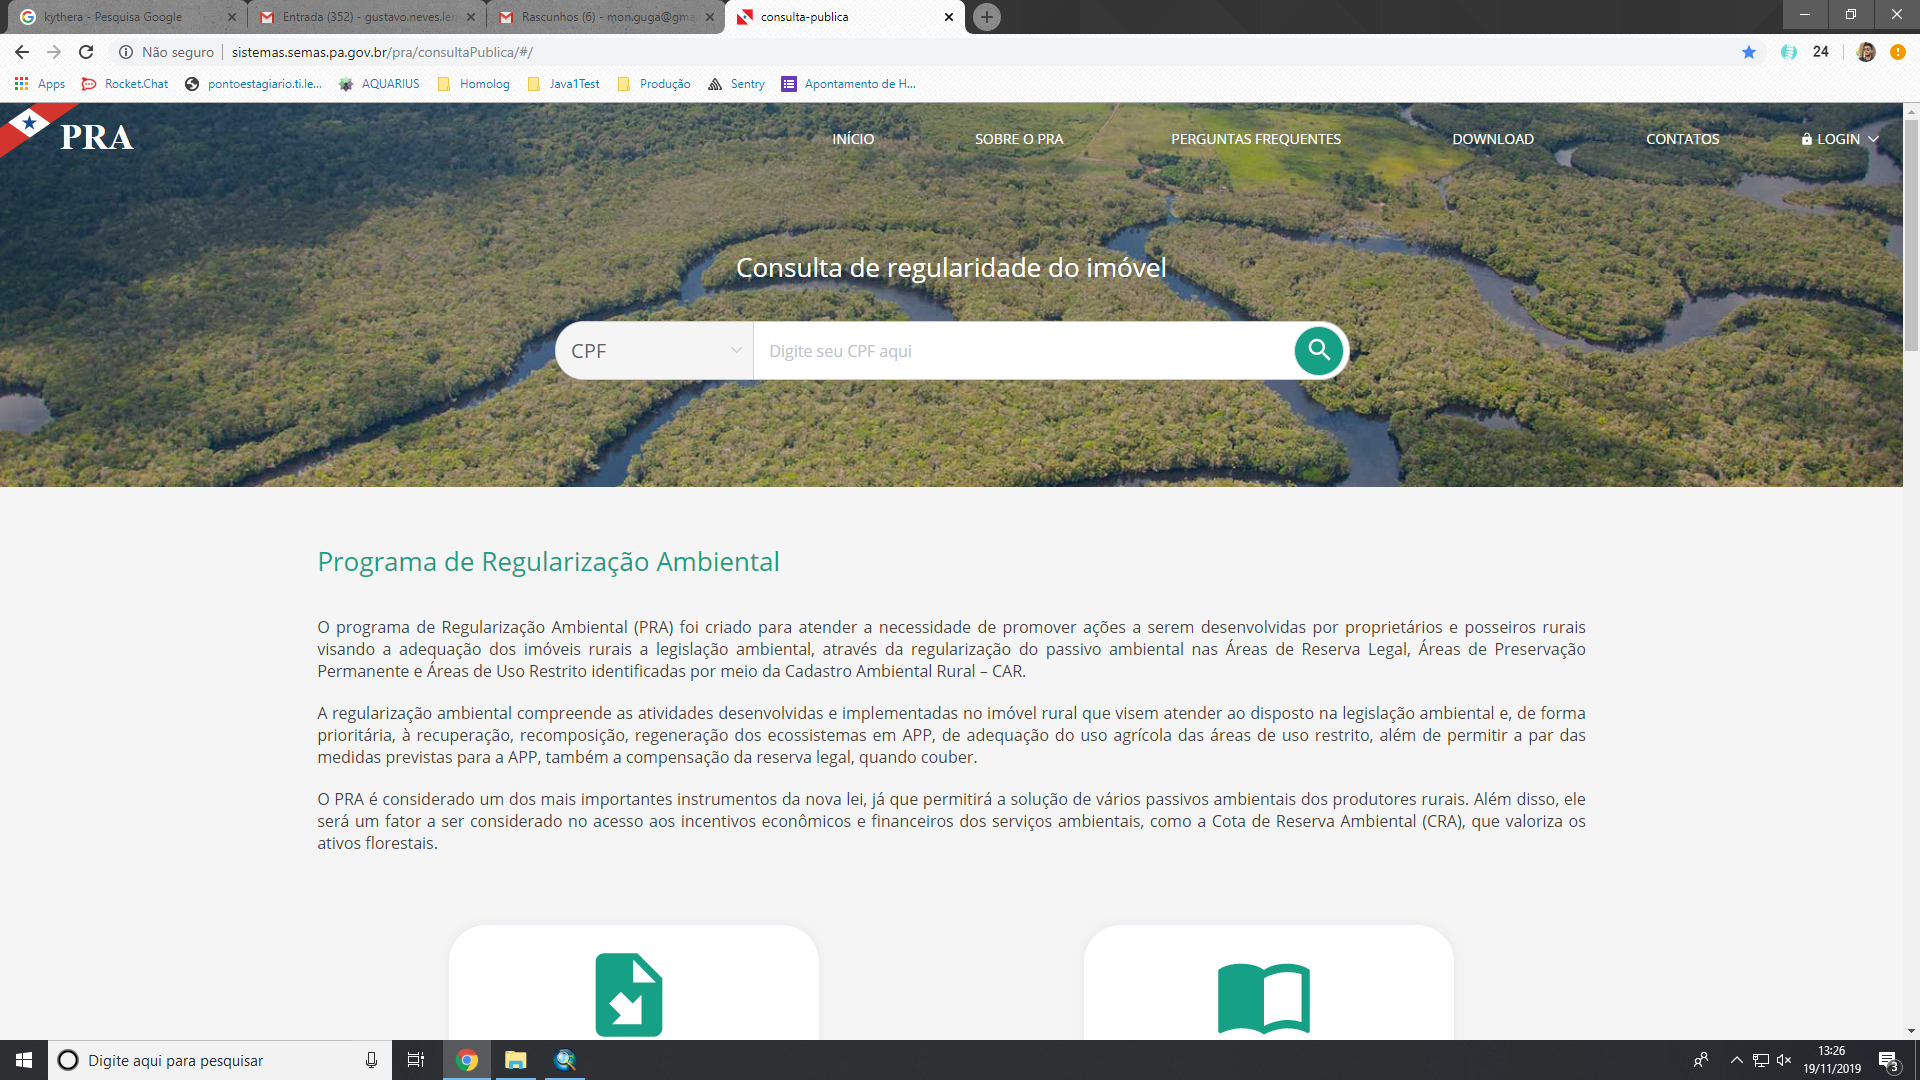
\includegraphics[scale=0.22]{consulta-publica}\\  % o 0.9 indica 90% do tamanho original
% pdfLaTeX aceita figuras no formato PNG, JPG ou PDF
% figuras vetoriais podem ser exportadas para eps e depois convertidas para pdf usando epstopdf
{\small Fonte: \url{http://sistemas.semas.pa.gov.br/pra/consultaPublica/#/}} %Fonte da imagem
\label{fig:consultaPublica} %rotulo para refencia
\end{figure}

O projeto Consulta Pública(Figura \ref{fig:consultaPublica}) foi o primeiro projeto que tive como atividade a refatoração, pois se tratava de um projeto legado, utilizava uma das primeiras versões de VueJS no \textit{frontend} e tinha o layout bem ruim.
Foi a primeira obrigação que tive total responsabilidade, pois tinha que migrar todo o sistema para VueJS 2.0 e refatorar o \textit{frontend}.

Como era sua primeira experiência com o \textit{framework} VueJS, foi demandado mais tempo do que o usual, mas tive suporte do meu time que me auxiliava sobre arquitetura, padrões de projetos e boas práticas de programação.
Para melhor aprendizado e controle sobre códigos ruins, todas modificações feitas por mim eram submetidas ao Code Review\footnote{Revisão do código, consiste em algum ou alguns membros da equipe analisando meu código e fazendo comentários de melhorias} enviadas para o projeto apenas perante aprovação. 

O projeto Consulta Pública tinha como objetivo ilustrar aos proprietários de imóveis rurais suas áreas desmatadas, se seus imóveis estavam ou não de acordo com as regularizações ambientais e informações gerais sobre a geometria e hidrografia do terreno.

\begin{figure}[H]
\centering
\caption{Relatórios do PRA} %legenda
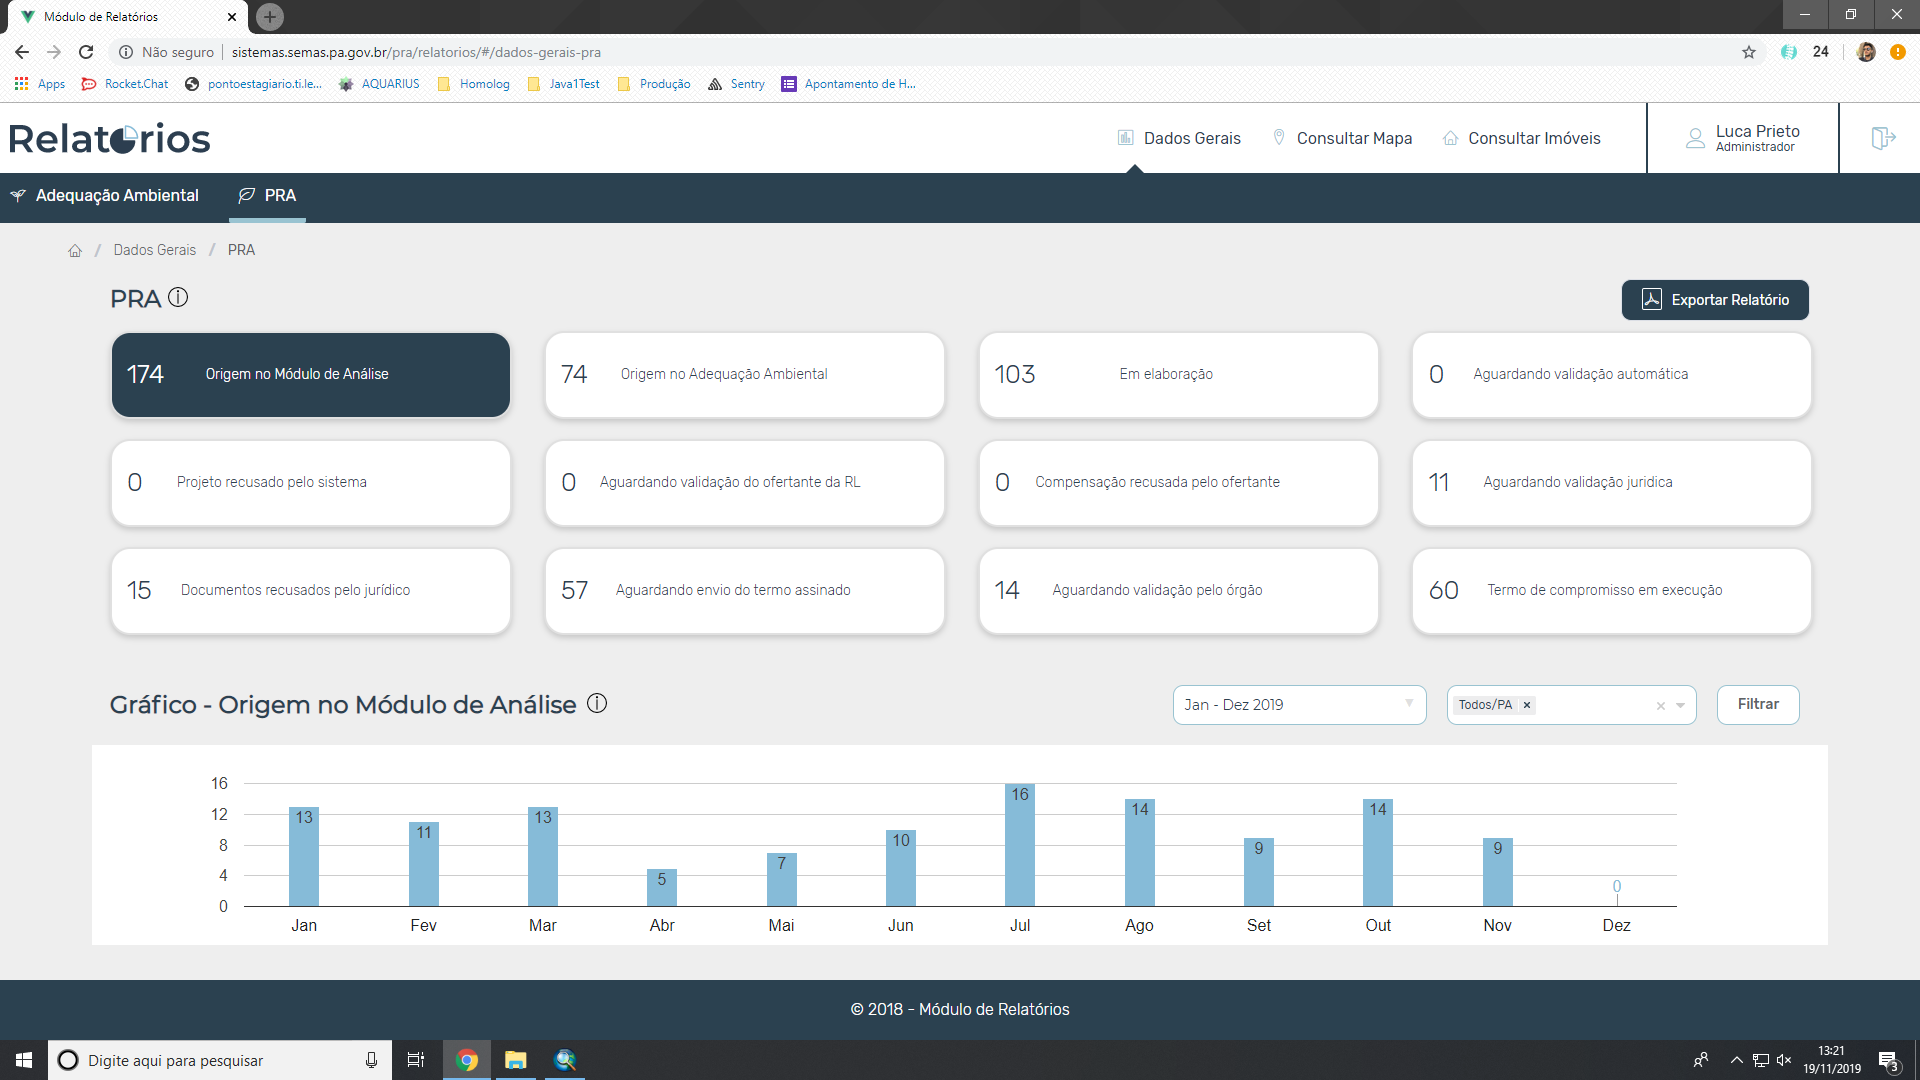
\includegraphics[scale=0.22]{relatorios-pra}\\  % o 0.9 indica 90% do tamanho original
% pdfLaTeX aceita figuras no formato PNG, JPG ou PDF
% figuras vetoriais podem ser exportadas para eps e depois convertidas para pdf usando epstopdf
{\small Fonte: \url{http://sistemas.semas.pa.gov.br/pra/relatorios/#/dados-gerais-adequacao-ambiental}} %Fonte da imagem
\label{fig:relatorios} %rotulo para refencia
\end{figure}

\section{Relatórios do PRA}
O projeto de relatórios(Figura \ref{fig:relatorios}) foi o primeiro projeto que tive participação desde o início, com uma equipe formada de 4 pessoas (2 desenvolvedores, uma tester e uma PO).
O projeto consistia em uma plataforma de relatórios sobre o Programa de Regularização Ambiental e Adequação Ambiental.

Foi o primeiro momento que tive que realmente aprender e utilizar dos conhecimentos relacionados a Banco de dados, e como havia feito a disciplina de Banco de Dados 1 e estava cursando Banco de Dados 2, foi de extrema importância os aprendizados das mesmas,
uma vez que lhe foi explicado melhor como funcionava os bancos e até mesmo como funcionava os bancos relacionados a geometrias espaciais.

O time tive autonomia de escolha da tecnologia, então pela ótima experiência com VueJS e o alto desempenho de tal, este foi o escolhido para o \textit{frontend}.
Porém, pelo baixo conhecimento sobre \textit{backend}, a escolha da tecnologia foi feita pelo outro desenvolvedor da equipe, que escolheu Spring Boot.
Como sua experiência se limitava apenas a evolução de software, houve diversos gargalos no desenvolvimento, como criação de ambientes, scripts para automatização de deploy entre outros.

Em meio a este projeto, descobriram um problema gigantesco no primeiro sistema que tive contato, o PRA-OFF. Ele quem empacotava e compactava as geometrias para o arquivo .PRA, porém, quando existiam muitas geometrias, o arquivo PRA podia ter tamanhos acima de 1GB.
O outro módulo, central do Responsável Técnico, que recebia os arquivos PRA, não aguentava processar o arquivo, travando no envio do mesmo.

Foi então sua responsabilidade desenvolver uma solução prática para o mesmo. Ná época, estava cursando a matéria de Programação Paralela e Concorrente, daí tive a ideia de otimizar este processo atravez de threads e processos, porém só isso não resolvia o problema.
Após liberar bastante poder de processamento para o servidor e criar diversas otimizações no processo de criação do PRA, foi possível diminuir o arquivo para aproximadamente 1/4 de meu tamanho original.

Isso se tornou possível através de consultas a pessoas mais experientes com dados geográficos, que me sugeriram converter as geometrias de GEOMETRY para KML.

Mas após 2 meses, por necessitarem de um desenvolvimento com maior domínio de \textit{frontend}, fui transferido para uma equipe especial, pois a tal não possuía tribo determinada.
O projeto era uma POC (Prova de conceito) direcionada a uma empresa do ramo de agronomia. Com prazos curtíssimos e complexidade alta, o projeto foi um dos mais difíceis que já trabalhei.
O projeto foi construído utilizando componentização, com o \textit{backend} feito com uma arquitetura bem definida e documentada para que fosse possível evoluir com o menor nível de dificuldade possível. Devido ao começo bem estruturado e documentado, o projeto foi bem sucedido.

Após esse projeto, fui alocado na tribo Atlântida, onde trabalhei juntamente com mais um desenvolvedor em no projeto SEIRH-CMS.

\section{SEIRH-CMS}

O projeto do SEIRH-CMS(Figura \ref{fig:seirhCms}) era um gerenciador de conteúdo da aplicação SEIRH\footnote{Sistema Estadual de Informações Sobre Recursos Hídricos do Pará, responsável sobre oferecer informações sobre os projetos e programas relacionados a recursos hídricos do pará}.
\begin{figure}[H]
\centering
\caption{SEIRH-CMS} %legenda
\includegraphics[scale=0.22]{SEIRH-CMS}\\  % o 0.9 indica 90% do tamanho original
% pdfLaTeX aceita figuras no formato PNG, JPG ou PDF
% figuras vetoriais podem ser exportadas para eps e depois convertidas para pdf usando epstopdf
{\small Fonte: \url{http://monitoramento.semas.pa.gov.br/SEIRHCMS}} %Fonte da imagem
\label{fig:seirhCms} %rotulo para refencia
\end{figure}
A plataforma web do SEIRH(Figura \ref{fig:seirh}) já existia, porém não havia comunicação com um \textit{backend}, então meu conteúdo não era gerenciável. Logo, havia a necessidade de refatoração total do sistema.

\begin{figure}[H]
\centering
\caption{SEIRH} %legenda
\includegraphics[scale=0.22]{SEIRH}\\  % o 0.9 indica 90% do tamanho original
% pdfLaTeX aceita figuras no formato PNG, JPG ou PDF
% figuras vetoriais podem ser exportadas para eps e depois convertidas para pdf usando epstopdf
{\small Fonte: \url{http://monitoramento.semas.pa.gov.br/SEIRH}} %Fonte da imagem
\label{fig:seirh} %rotulo para refencia
\end{figure}

Então, a refatoração do sistema foi atribuída como tarefa designada ao nosso time.
Como meu conhecimento sobre \textit{backend} já era mais amplo e devido a tribo Atlântida ser constituída de desenvolvedores DotNet, resolvemos utilizar o \textit{framework} DotNet Core 2.0, que 
provia diversas funcionalidades e atendia as nossas expectativas e necessidades.
Já o \textit{frontend} continuou sendo feito com VueJS, uma vez que nossas experiências com tal \textit{framework} eram recentes.

O prazo para entrega do projeto era curtíssimo de duas \textit{Sprints}(1 mês), então optamos por utilizar um quadro \textit{Kanban} para gerenciar as atividades.
Esta foi sua primeira experiência exercendo liderança em estabelecer as prioridades e definir as atividades, definição das atividades e organização no geral.

O projeto foi finalizado com excelência e no prazo estipulado, o que me rendeu nova oportunidade de alocação em um time que já trabalhava com DotNet e necessitava de mais um desenvolvedor.

O projeto desta vez fazia parte de um grande complexo de plataformas que havia sido encomendado por uma empresa de agronomia e tinha muitos componentes de \textit{frontend} similares entre sí.

Desse fato ocorreu uma iniciativa sua e de outro desenvolvedor de iniciarmos a construção do Design System em um contexto organizacional.

\section{Cria Design System}
Surgiu então, o Cria Design System(Figura \ref{fig:criaDesign})\footnote{Disponível em \url{https://criatecnologiainovacao.github.io/cria-design-ReactJS/}}, que é uma biblioteca de componentes UI\footnote{User Interface Design - é uma área de design que planeja e analisa os modos de iteração do usuario com o sistema.} para ReactJS.

Todos os componentes eram criados pelo design do projeto, definindo comportamentos e animações, desenvolvidos depois. Para a visualização individual dos componentes, utilizamos o StoryBook\footnote{Disponivel em: \url{https://storybook.js.org/}},
que cria e organiza o catálogo de componentes e então, para compartilhar tal biblioteca para toda a empresa e para que não surgissem bugs, foram implementados testes automatizados, 
uma vez que já havia tido contato com testes automatizados na disciplina de Engenharia de Software, e havia sido encorajado a desenvolver os mesmo em Desenvolvimento Web, resolvi que seria interessante a criação de testes de componentes, testando visualmente e comportamentalmente,
todos componentes e com necessidade mínima de cobertura de 80\%.

\begin{figure}[H]
\centering
\caption{Cria Design System} %legenda
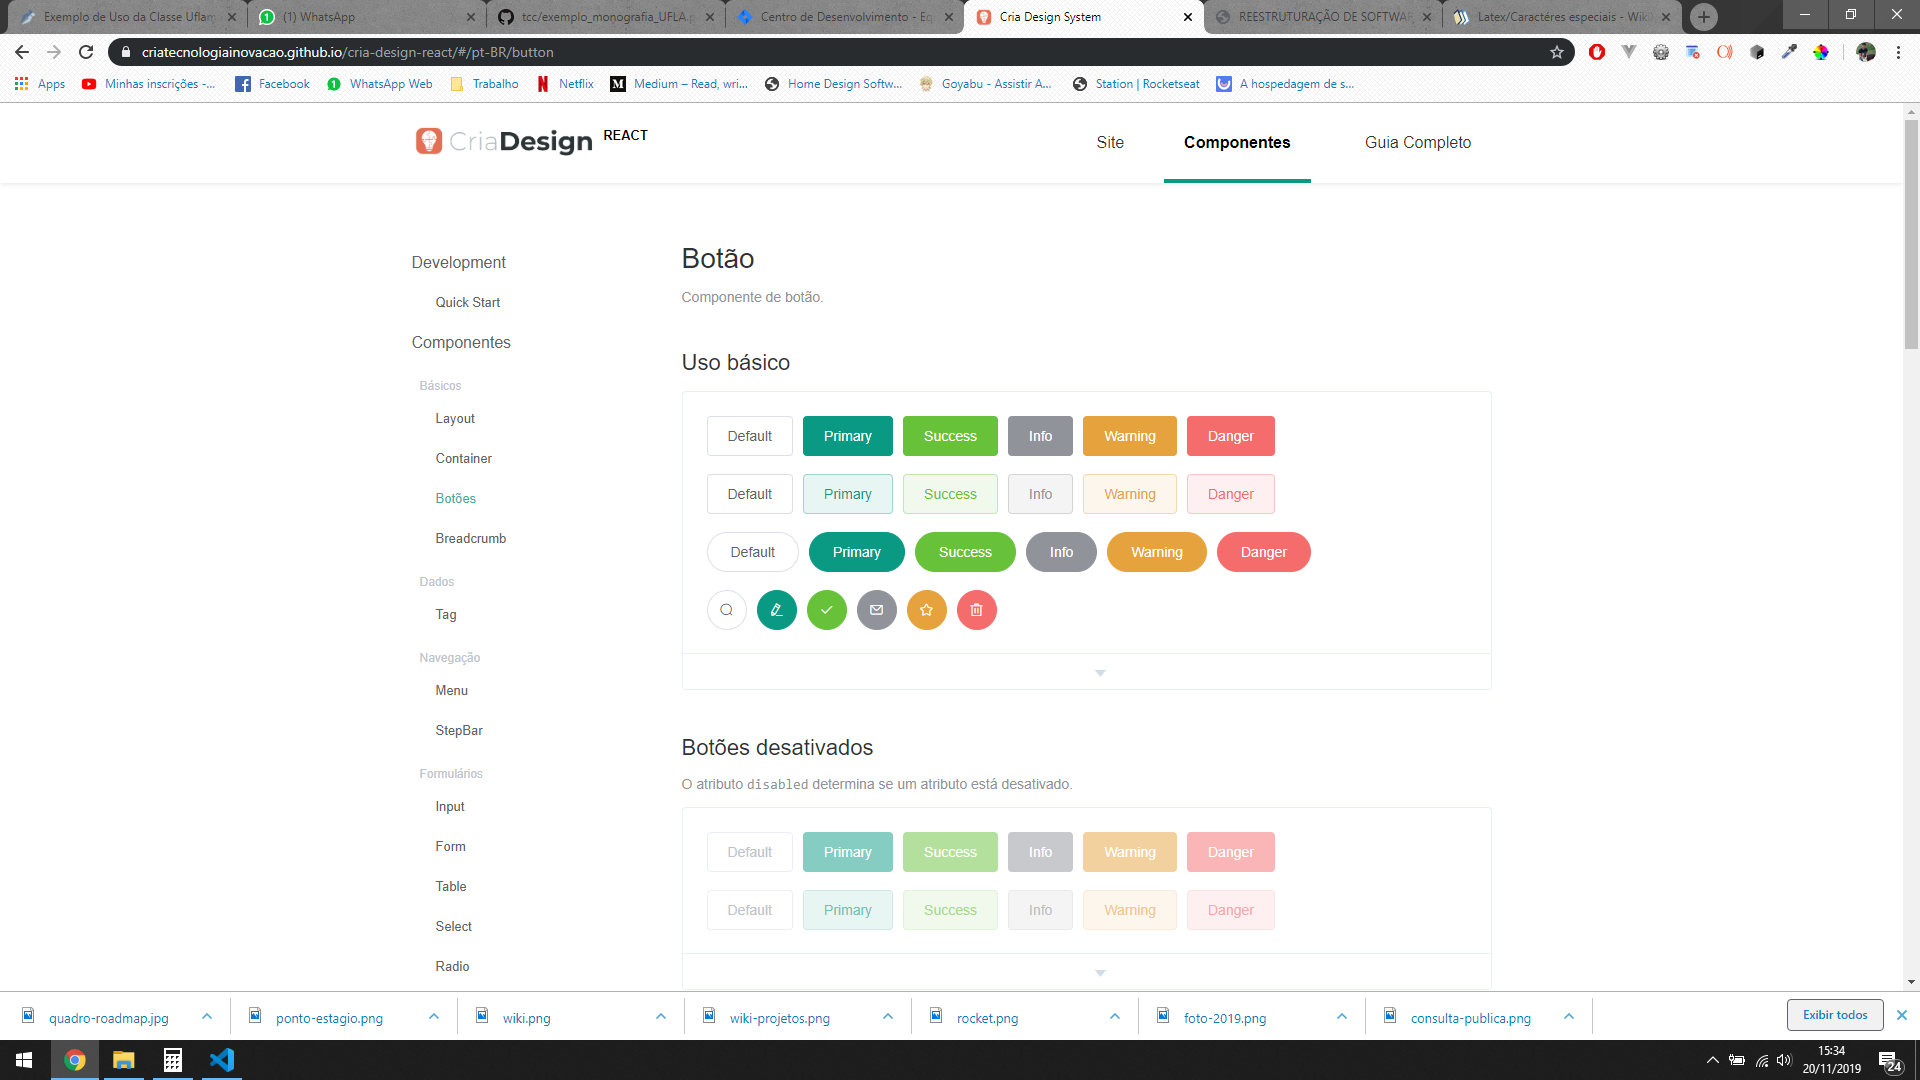
\includegraphics[scale=0.3]{cria-design}\\  % o 0.9 indica 90% do tamanho original
% pdfLaTeX aceita figuras no formato PNG, JPG ou PDF
% figuras vetoriais podem ser exportadas para eps e depois convertidas para pdf usando epstopdf
{\small Fonte: \url{https://criatecnologiainovacao.github.io/cria-design-ReactJS/}} %Fonte da imagem
\label{fig:criaDesign} %rotulo para refencia
\end{figure}

Após auxiliar com o início do projeto e facilitar o desenvolvimento do mesmo, fui incorporado a uma equipe da mesma tribo, que cuidava de alguns projetos como o SIOUT e SIGERH-PA.

\section{SIGERH-PA}

O projeto do SIGERH-PA(Figura \ref{fig:sigerhpa}) (Sistema de Gerenciamento de Recursos Hídricos do Pará) é uma plataforma de cadastro e regularização de recursos hídricos (poços artesianos, nascentes e outros).
Nele usávamos como \textit{backend} o \textit{framework} DotNet \textit{Framework} 4.0 e como \textit{frontend} AngularJS.

\begin{figure}[H]
\centering
\caption{SIGERHPA} %legenda
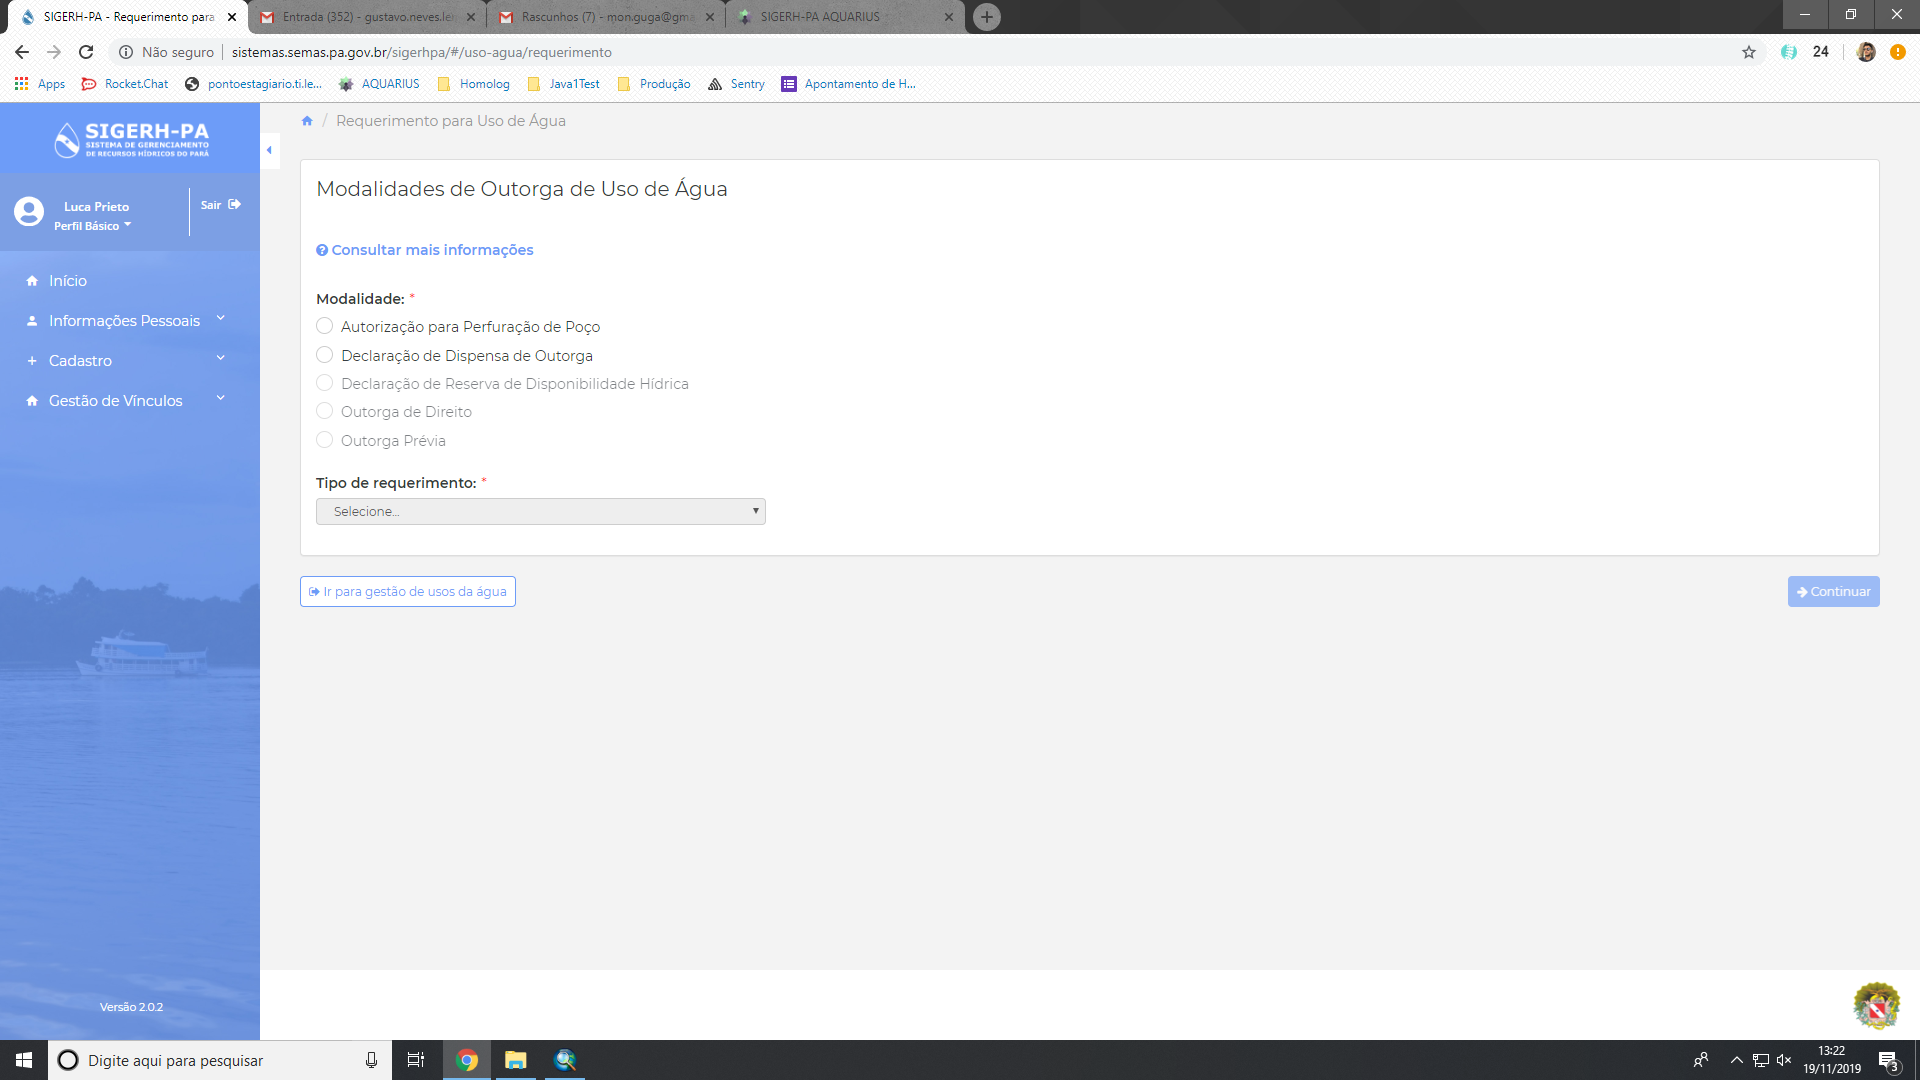
\includegraphics[scale=0.222]{sigerpa}\\  % o 0.9 indica 90% do tamanho original
% pdfLaTeX aceita figuras no formato PNG, JPG ou PDF
% figuras vetoriais podem ser exportadas para eps e depois convertidas para pdf usando epstopdf
{\small Fonte: \url{http://sistemas.semas.pa.gov.br/sigerhpa/}} %Fonte da imagem
\label{fig:sigerhpa} %rotulo para refencia
\end{figure}

O sistema tinha complexidade gigantesca, uma vez que para cada tipo de recurso hídrico, era necessário um fluxo especifico de cadastro.

Uma das atividades mais importantes que fui responsável foi o desenvolvimento de um novo fluxo, totalmente diferente dos outros, então o reaproveitamento de código foi baixíssimo, somente pude reaproveitar alguns componentes.
Ao final do meu estágio, tive como tarefas principais: aprimorar e corrigir tal sistema, que tinha
vários problemas, se tratando de um sistema bastante grande.